\documentclass{ximera}



%\newcommand{\pt}[1]{\leavevmode\marginnote[\hfill\textbf{/#1}]{\hfill/#1}\addtocounter{totaantal}{#1}}


\begin{document}
        \author{Bert Lambregs}
        \xmtitle{Oefeningen (per bestand)}



\begin{exercise}
% !TEX root = ../main.tex



 Beargumenteer het gebruik van het model van een eenparig versnelde beweging (EVB) voor de vrije beweging van een wagentje op een helling. Denk daarbij aan een proefneming die we in de klas deden. De notie kracht moet je hier even buiten beschouwing laten.

\begin{oplossing}

Het model beschrijft de meetgegevens accuraat.

M.a.w. zijn de meetgegevens van de positie van het wagentje op de helling in functie van de tijd, gemeten met een (ultrasone) positiesensor, accuraat te beschrijven met de plaatsfunctie van een eenparig versnelde beweging.

\emph{Toelichting}.
De vraag gaat over de relatie tussen de theorie en de realiteit. Het is maar door metingen te doen dat we kunnen nagaan of gevolgen van de theorie (in dit geval bijvoorbeeld dat de positie kwadratisch in de tijd verloopt voor een beweging met constante versnelling) overeenkomen met de realiteit. In het gegeven geval van een wagentje op een helling, is bijvoorbeeld een model van constante snelheid niet van toepassing. Het zou immers impliceren dat het wagentje niet van zin kan veranderen. Dat laatste wordt door metingen of waarnemingen weerlegd.

\end{oplossing} 

\end{exercise}
 % Model EVB wagentje op een helling
% 
\begin{exercise}
 Welke vectorvoorstelling stelt een EVRB voor die vertraagt naar de oorsprong van de $x$-as toe? Beargumenteer kort je keuze.
\begin{figure}[h]
\centering
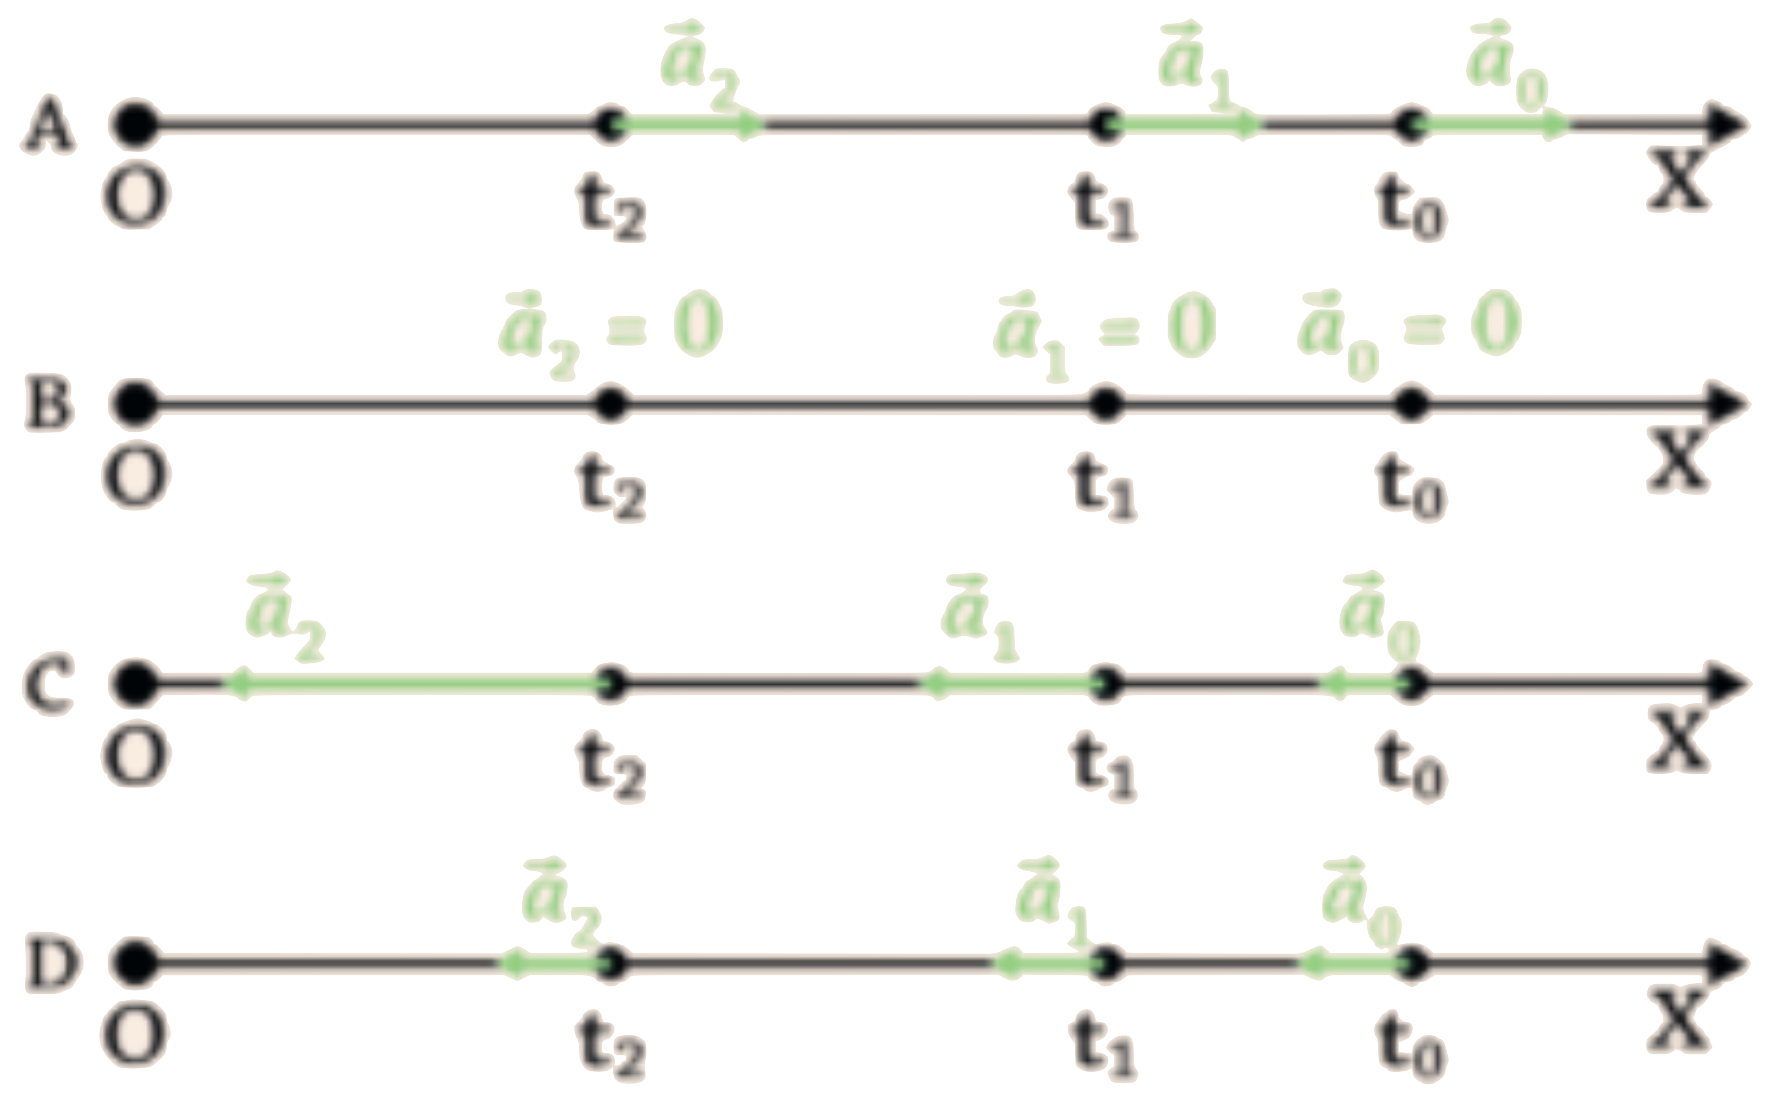
\includegraphics[width=0.8\textwidth]{18p40}
\end{figure}

\end{exercise}
 % Meerkeuze Oriëntatie versnelling

\begin{exercise}
% !TEX root = ../main.tex


 Toon aan dat de positie en de snelheid van een eendimensionale beweging met constante versnelling gegeven worden door de volgende functies:
\begin{align*}
    x(t)&=x_0+v_0t+\frac{1}{2}at^2\\
    v(t)&=v_0+at 
\end{align*}

\end{exercise}
 % Formules EVRB

\begin{exercise}
% !TEX root = ../main.tex




 Een auto vertrekt vanuit rust en bereikt na \SI{3,0}{km} een snelheid van \SI{450}{km/h} We onderstellen de versnelling constant en de baan recht. Bereken de versnelling en de tijd, nodig om die \SI{3,0}{km} af te leggen.
\begin{oplossing}
    % \item[gegeven]$x=3000\rm\,m$\newline $v=125\rm\,m/s$
    % \item[gevraagd]$a$, $t$
    % \item[oplossing]
    Omdat voor een EVRB de gemiddelde snelheid gegeven wordt door $\overline{v}=\frac{v_0+v}{2}$ en we de afgelegde afstand kennen, kunnen we de benodigde tijd gemakkelijk vinden. We kiezen $t_0=0$, $x_0=0$. De beginsnelheid is nul zodat:
    \begin{eqnarray*}
        \Delta x &=& \overline{v}\Delta t \\
        &\Downarrow & \\
        t &=& \frac{x}{\left(\frac{v}{2}\right)} = \frac{2x}{v}
    \end{eqnarray*}
    Invullen van de gegevens levert een tijd van \SI{48}{s}. Met de formule $v=v_0+at$ voor de snelheid vinden we de versnelling door de tijd erin te substitueren, en de beginsnelheid nul te nemen:
    \begin{eqnarray*}
        % v &=& at \\
        % &\Updownarrow&\\
        a &=& \frac{v}{t}=\frac{v}{\left(\frac{2x}{v}\right)}\\
        &=& \frac{v^2}{2x}
    \end{eqnarray*}
    Invullen van de gegeven grootheden levert een versnelling van \SI{2,6}{m/s^2}.
\end{oplossing}

\end{exercise}

\item Bewijs voor een eenparig veranderlijke rechtlijnige beweging (EVRB) de volgende formule voor de gemiddelde snelheid:
\begin{equation*}
    \overline{v}=\frac{v_0+v}{2}
\end{equation*} % Bewijs formule gemiddelde snelheid
% !TEX root = ../main.tex


\item\pt{4}Een massa vertrekt vanuit rust om een EVB uit te voeren. Als haar beginpositie \SI{0}{m} is, welke van de volgende betrekkingen is dan juist? Toon aan
\newline
\newline
\begin{tabularx}{\textwidth}{XXXX}
	(a) $t=\frac{x}{2v}$&(b) $t=\frac{2x}{v}$&(c) $t=\frac{v}{2x}$&(d) $t=\frac{2v}{x}$
\end{tabularx}

\begin{oplossing}
(b)
\end{oplossing}
 % Eenvoudige algebra met formules EVB

\begin{exercise}
% !TEX root = ../main.tex


[\SI{80}{\percent} (b)] Een vliegtuig start vanuit rust en versnelt met een constante versnelling langs de grond alvorens op te stijgen. Het legt \SI{600}{m} af in \SI{12}{s}. Bepaal de versnelling, de snelheid na \SI{12}{s} en de afstand afgelegd gedurende de twaalfde seconde.

\begin{oplossing}
	$a=\frac{2x}{t^2}=\SI{8,33}{m/s^2}$,
	$v=\frac{2x}{t}=\SI{100}{m/s}$,
	$x(t=12)-x(t=11)=\frac{1}{2}a(t_{12}^2-t_{11}^2)=\SI{95,8}{m}$
\end{oplossing}


\end{exercise}
 % Vliegtuig, Afstand gedurende 12e seconde
% !TEX root = ../main.tex


\item\pt{4}Kan de snelheid van een voorwerp gelijk zijn aan nul, terwijl de versnelling verschillend is van nul? Motiveer je antwoord.

\begin{exercise}
% !TEX root = ../main.tex


\pt{4}Kan de bewegingsrichting van een voorwerp omkeren terwijl de versnelling gelijk blijft? Zo ja, geef dan een voorbeeld. Zo nee, leg uit waarom dat niet kan.

\begin{oplossing}
Ja, dat kan. Als je een bal opwerpt zal op het hoogste punt de bewegingszin omdraaien terwijl de versnelling gelijk blijft. We kunnen immers een verticale worp modelleren als een EVB. Kiezen we de referentieas om de beweging te beschrijven omhoog, dan is de snelheid van de bal positief bij het naar boven bewegen en negatief wanneer hij naar beneden komt, terwijl de verandering van de snelheid in de tijd (de versnelling) systematisch gelijk is aan de negatieve valversnelling.


ChatGPT:

Ja, de bewegingsrichting van een voorwerp kan omkeren terwijl de versnelling gelijk blijft. Dit gebeurt wanneer de versnelling tegengesteld is aan de bewegingsrichting van het voorwerp. In zo'n geval zal het voorwerp eerst vertragen totdat het stopt, en daarna versnellen in de tegenovergestelde richting.

\textbf{Voorbeeld:}

Stel je voor dat je een bal recht omhoog gooit. De zwaartekracht zorgt voor een constante versnelling naar beneden (ongeveer \SI{9,8}{m/s^2}). Terwijl de bal omhoog beweegt, is de snelheid van de bal naar boven gericht, maar de versnelling door de zwaartekracht blijft naar beneden gericht.

\begin{itemize}
\item Op het hoogste punt komt de bal kort tot stilstand (de snelheid is nul), maar de versnelling naar beneden verandert niet.
\item Na dat punt keert de bal om en begint naar beneden te vallen, met een toenemende snelheid in de richting van de versnelling (naar beneden).
\end{itemize}

In dit scenario keert de bewegingsrichting van de bal om van omhoog naar omlaag, terwijl de versnelling constant naar beneden blijft gericht.


\end{oplossing}


\end{exercise}

% !TEX root = ../main.tex


\item\pt{4}Kan een voorwerp dat een positieve versnelling heeft een negatieve snelheid hebben? Kan het omgekeerde ook? Licht je antwoord toe.

\begin{oplossing}
    Ja, dat kan. Neem bijvoorbeeld een voorwerp dat je verticaal omhoog gooit. Als je de referentieas waarmee je de beweging wil beschrijven verticaal naar benden kiest, zal de versnelling van de beweging positief zijn en de snelheid negatief. De snelheid is negatief omdat je tegengesteld aan de as beweegt en de versnelling is positief omdat de snelheid minder negatief wordt.

    Het omgekeerde kan ook, draai gewoon de referentieas om.
\end{oplossing}
% 
\begin{exercise}
% !TEX root = ../main.tex


\pt{4}In de figuur zie je zes bewegingen van een bal die van links naar rechts beweegt. De pijlen geven de positieve richting oftewel de $x$-as aan. Elke cirkel stelt de positie van de bal voor op opeenvolgende tijdstippen. De tijdsintervallen tussen die opeenvolgende tijdstippen zijn gelijk.
\begin{figure}[hbt]
	\begin{flushright}
	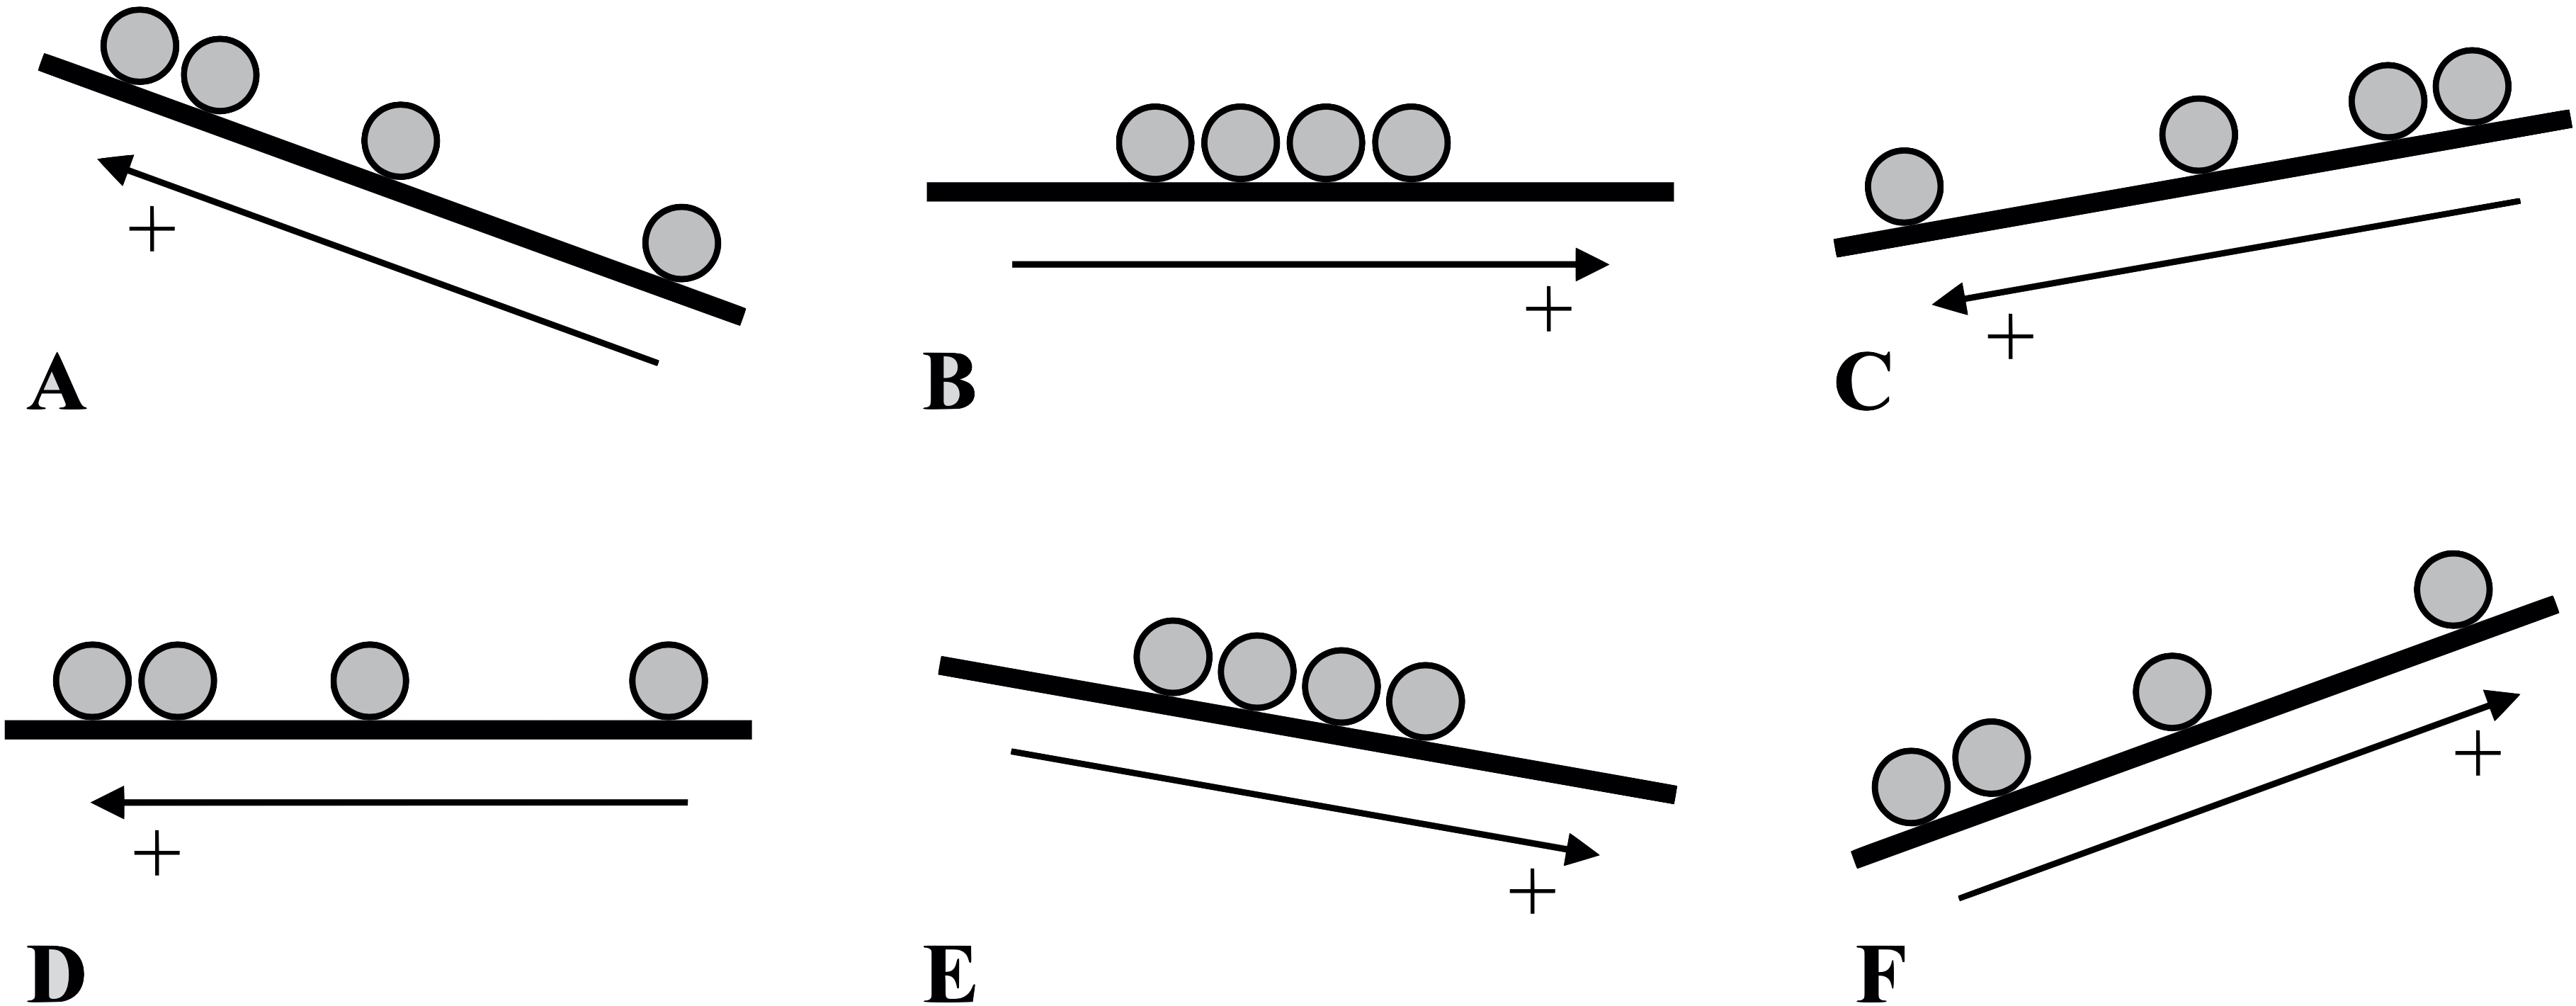
\includegraphics[width=.93\textwidth]{hb_natuurkundedidactiek_34}
	%\includegraphics[height=\textheight]{}
	%\caption{}
	\end{flushright}
\end{figure}
\begin{enumerate}
\item Zet de bewegingen op volgorde op basis van de eindsnelheid van de bal. Begin met de beweging waarbij die eindsnelheid het grootst is. Let op: nul is groter dan negatief.
\item Doe hetzelfde als in (a) maar nu voor de versnelling van de bal.% (in plaats van de eindsnelheid). %Zet de bewegingen op volgorde op basis van de versnelling van de bal. Begin met de beweging waarbij die versnelling het grootst is. Let op: nul is groter dan negatief.
\end{enumerate}
Als er twee of meer situaties zijn die gelijk ‘scoren’, dan komen die situaties op dezelfde plaats in jouw volgorde te staan. Je geeft dat aan door ze bijvoorbeeld te omcirkelen. %Leg ten slotte de redenering achter jouw volgorde uit.

\begin{oplossing}
	(a) F, B=E, C, A=D
	
	(b) F=C, B=E, A=D
\end{oplossing}

\end{exercise}
 % Ordenen snelheid en versnelling
% !TEX root = ../main.tex


\item[\SI{80}{\percent} (b)]Vanop een grote hoogte laat men achtereenvolgens twee stenen vallen met een tussentijd van 2 seconden. Op welke wijze verandert de afstand tussen beide stenen in de tijdsduur dat beide vallen? (Begin met een grafische voorstelling.) 

\begin{oplossing}
	De afstand verandert lineair in functie van de tijd: $\Delta x(t)=gt_0\cdot t-\frac{1}{2}gt_0^2$ ($=\frac{1}{2}gt^2-\frac{1}{2}g(t-t_0)^2$ met $t\geq t_0=\SI{2}{s}$)
\end{oplossing} % Verloop afstandsverschil vallende lichamen
% !TEX root = ../main.tex


\pt{4}\begin{minipage}[t]{.6\linewidth}
	Teken de overeenkomstige $x(t)$- en $a(t)$-grafiek bij de gegeven $v(t)$-grafiek. Ga ervan uit dat $x_0=\SI{0}{m}$.
\end{minipage}
\hfill
\begin{minipage}[t]{.37\linewidth}
	\raisebox{1ex-\height}{%
		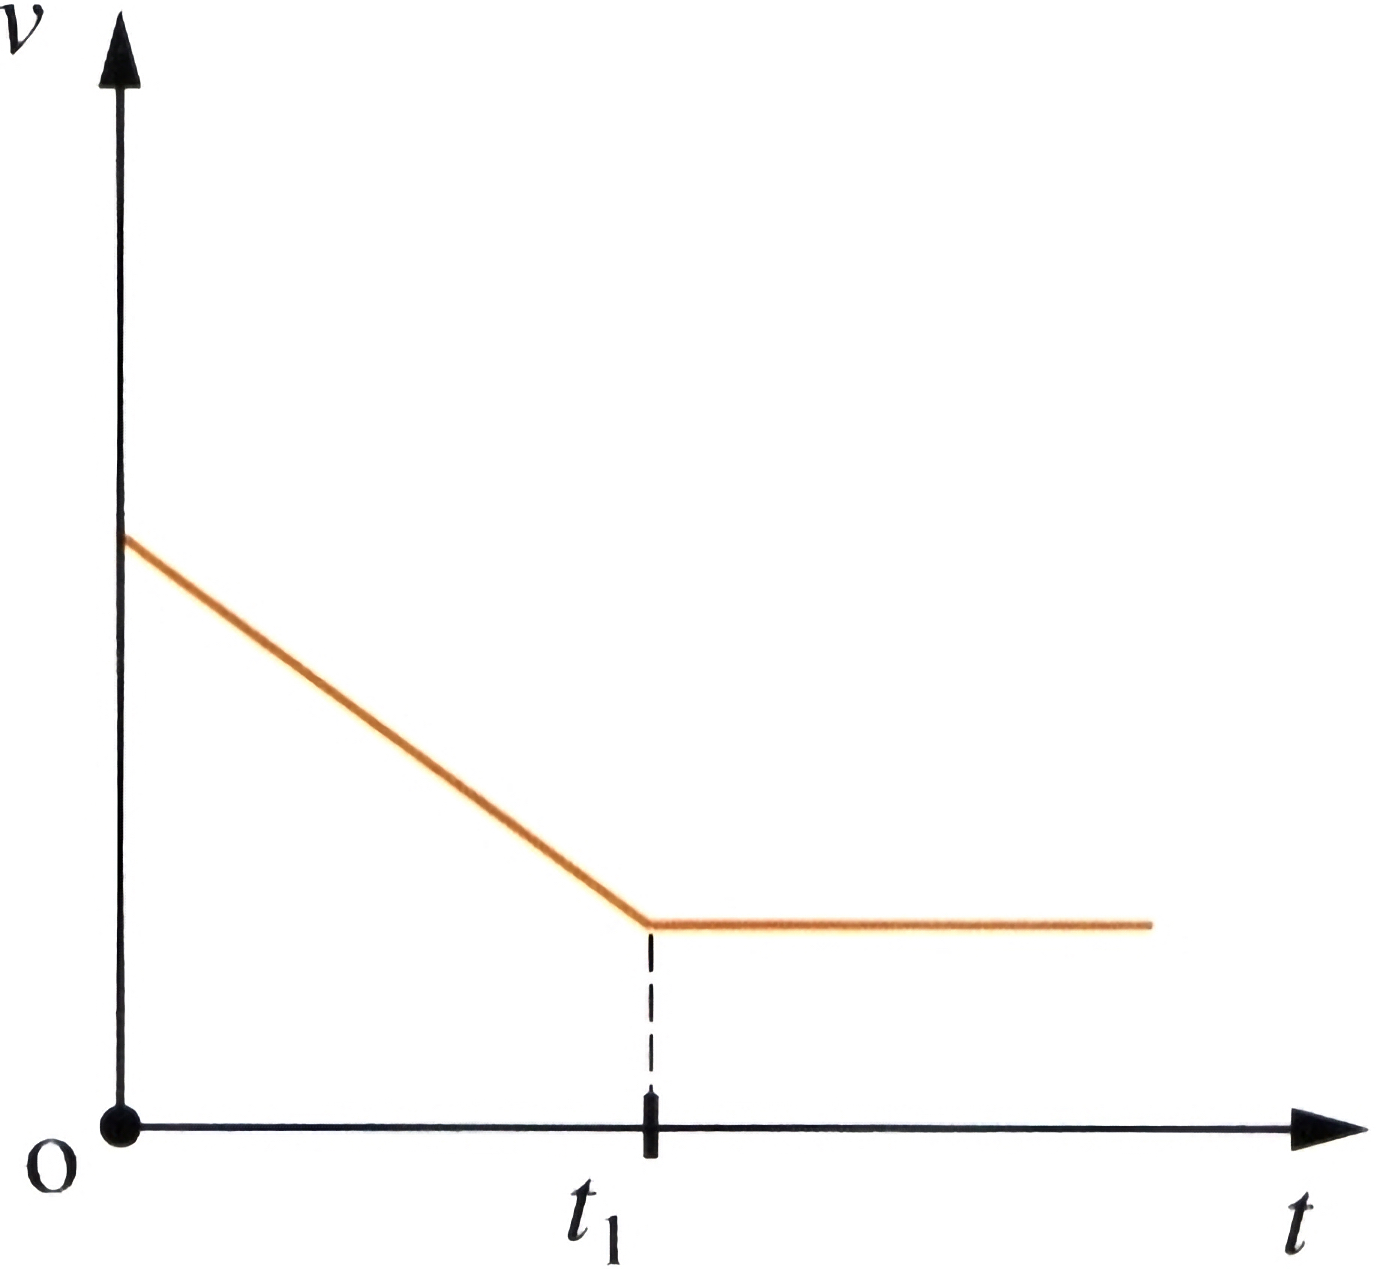
\includegraphics[width=\textwidth]{v(t)}%
		} 
\end{minipage}
% 
\begin{exercise}
% !TEX root = ../main.tex


\pt{2}De snelheid van een deeltje voldoet aan $v=at$ waarin $a$ constant en negatief is. De plaats van het deeltje wordt voorgesteld door $x$. Aangenomen wordt dat $x=0\rm\,m$ op het ogenblik $t=0\rm\,s$. Welke grafiek geeft het juiste verloop van $x(t)$?
\begin{figure}[h]
\begin{flushright}
%%TODO%%% \import{./img/}{30p38_a.tex}\import{./img/}{30p38_b.tex}
%\end{center}
%\begin{center}
%%TODO%% \import{./img/}{30p38_c.tex}\import{./img/}{30p38_d.tex}
%\caption{Caption}
%\label{fig:my_label}
\end{flushright}
\end{figure}

\begin{oplossing}
3e optie
\end{oplossing}


\end{exercise}

% 
\begin{exercise}
% !TEX root = ../main.tex



\pt{2}Een lichaam wordt verticaal omhoog geworpen. De referentieas is omhoog gericht. Welke van de volgende $v(t)$-diagrammen geeft dan het juiste verloop van de snelheid weer?
\begin{figure}[h]
\begin{flushright}
%%TODO%% 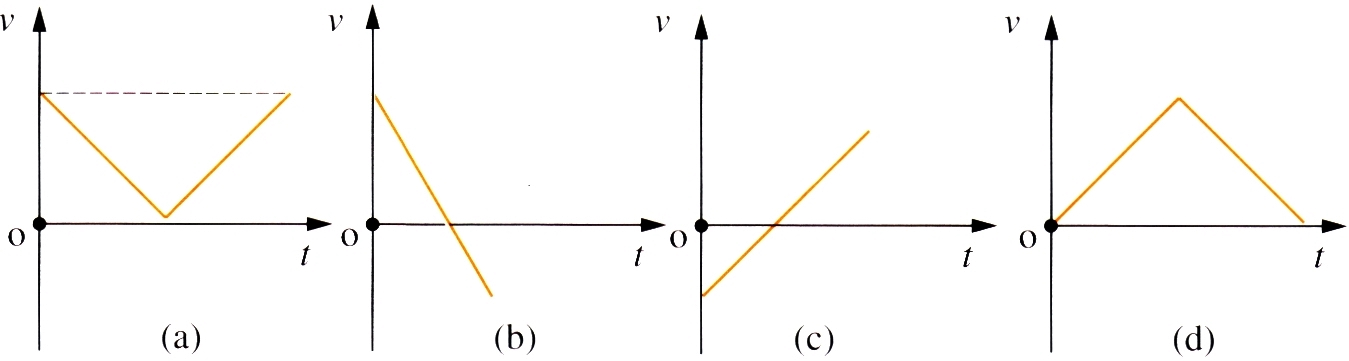
\includegraphics[width=0.93\textwidth]{vw}
\end{flushright}
\end{figure}

\begin{oplossing}
Het juist antwoord is (b). De versnelling is constant waardoor de snelheid lineair moet verlopen in de tijd. Aangezien de referentieas naar boven is gekozen, moet de snelheid in het naar boven bewegen positief zijn. Dat is het geval bij (b).
\end{oplossing}

\end{exercise}


\begin{exercise}
 Een trein met veel rijtuigen heeft een snelheid van \SI{100}{km/h} en komt over een afstand van \SI{520}{m} tot stilstand. Hoe groot is zijn versnelling?

\end{exercise}

% 
\begin{exercise}
% !TEX root = ../main.tex


[\SI{80}{\percent} (b)] Een trein rijdt tegen een snelheid van \SI{72}{km/h} en remt met een versnelling waarvan de grootte \SI{1,0}{m/s^2} bedraagt. Na hoeveel tijd komt de trein tot stilstand en welke afstand wordt er tijdens dit afremmen afgelegd?

\begin{oplossing}
    % \item[gegeven]$v_0=\SI{20}{m/s}\newline $a=\SI{-1,0}{m/s^2}
    % \item[gevraagd]$t$, $x$
    % \item[oplossing]
    Aangezien er per seconde een snelheid van \SI{1,0}{m/s} van de beginsnelheid afgaat, vinden we de tijd die nodig is voor het remmen, door de beginsnelheid te delen door de versnelling. Dat is namelijk de tijd die nodig is voor de trein om tot stilstand te komen:
    \begin{eqnarray*}
        v&=&0\\
        &\Updownarrow&\\
        v_0+at&=&0\\
        &\Updownarrow&\\
        t&=&-\frac{v_0}{a}
    \end{eqnarray*}
    Invullen van de gegevens levert een tijd van $20\rm\,s$. De afgelegde afstand gedurende het remmen vinden we nu met de plaatsfunctie. We kennen de benodigde tijd, die we in de plaatsfunctie invullen.\footnote{Een andere mogelijkheid is vertrekken met $x=\overline{v}t$}
    \begin{eqnarray*}
        x&=&v_0t+\frac{1}{2}at^2\\
        &=&v_0\left(-\frac{v_0}{a}\right)+\frac{1}{2}a\left(-\frac{v_0}{a}\right)^2\\
        &=&-\frac{v_0^2}{a}+\frac{v_0^2}{2a}\\
        &=&-\frac{v_0^2}{2a}\\
    \end{eqnarray*}
    Invullen van de gegevens levert een remafstand van \SI{200}{m}. 
\end{oplossing}

\end{exercise}
 % Remmende trein
% % !TEX root = ../main.tex


\pt{4}Laat zien dat voor een EVB waarvoor $x_0=0$ de volgende formule geldt:
\begin{eqnarray*}
v^2=v_0^2+2ax
%v^2=v_0^2+2a(x-x_0)
\end{eqnarray*}

\begin{oplossing}
Uit $v=v_0+at$ volgt:
\begin{eqnarray*}
v^2&=&v_0^2+2v_0at+a^2t^2\\
&=&v_0^2+2a(v_0t+\frac{1}{2}at^2)\\
&=&v_0^2+2ax
\end{eqnarray*}
\end{oplossing}
 % Formule v^2-v_0^2=2ax bewijzen
% % !TEX root = ../main.tex


\item\pt{2}De snelheid van een lichaam dat vanuit rust vrij valt, bedraagt na een valafstand $x$:
%De snelheid van een lichaam dat vrij valt vanuit rust, bedraagt na een valafstand $x$ (licht je antwoord toe):
%\newline
%\newline

\vspace{\baselineskip}
\begin{tabularx}{\textwidth}{XXXX}
(a) $v=2gx$&(b) $v=\sqrt{2gx}$&(c) $v=gx$&(d) $v=\sqrt{\frac{gx}{2}}$
\end{tabularx}

\begin{oplossing}
(b) $v=gt=g\sqrt{\frac{2x}{g}}=\sqrt{2gx}$
\end{oplossing}
 % mk
% % !TEX root = ../main.tex


\pt{10}Uit een punt op \SI{28,0}{m} boven de grond wordt een bal verticaal omhoog geworpen met een snelheid van \SI{12}{m/s}. Bepaal
\begin{enumerate}
\item de door het lichaam bereikte hoogte boven de grond;
\begin{oplossing}
\newline
$v=0\Leftrightarrow x=x_0+\frac{v_0^2}{2g}=\SI{35,34}{m}$	
\end{oplossing}
\item de tijd nodig om de grond te bereiken;
\begin{oplossing}
\newline
	$x=0\Leftrightarrow t=\frac{v_0+\sqrt{v_0^2+2gx_0}}{g}=\SI{3,91}{s}$
\end{oplossing}
\item de snelheid bij het bereiken van de grond.
\begin{oplossing}
\newline
	$v=-\sqrt{v_0^2+2gx_0}=\SI{-26,33}{m/s}$
\end{oplossing}
\end{enumerate} %Verticale worp, standaard
% % !TEX root = ../main.tex

% 3 p. 92
[\SI{80}{\percent} (b)] Een pijl wordt verticaal van de grond omhooggeschoten en bereikt na \SI{2,8}{s} het hoogste punt. Bepaal deze hoogte.
\begin{oplossing}
\item[Gegeven]\SI{2,8}{s}
\item[Gevraagd]$v_0$, $x_{max}$

\item[Oplossing]\begin{minipage}[t]{0.6\linewidth}
	Op het hoogste punt is de snelheid van de pijl nul. Aangezien we weten hoe lang hij onderweg is en de pijl per seconde \SI{9,81}{m/s^2} trager omhoog vliegt, kunnen we hieruit de beginsnelheid bepalen. 
	
	We kiezen de referentie-as met de oorsprong op de grond. De versnellingscomponent is dan het tegengestelde van de valversnelling, $a=-g$.
\end{minipage}%
\begin{minipage}[t]{0.37\linewidth}
	\raisebox{1ex-\height}{%
	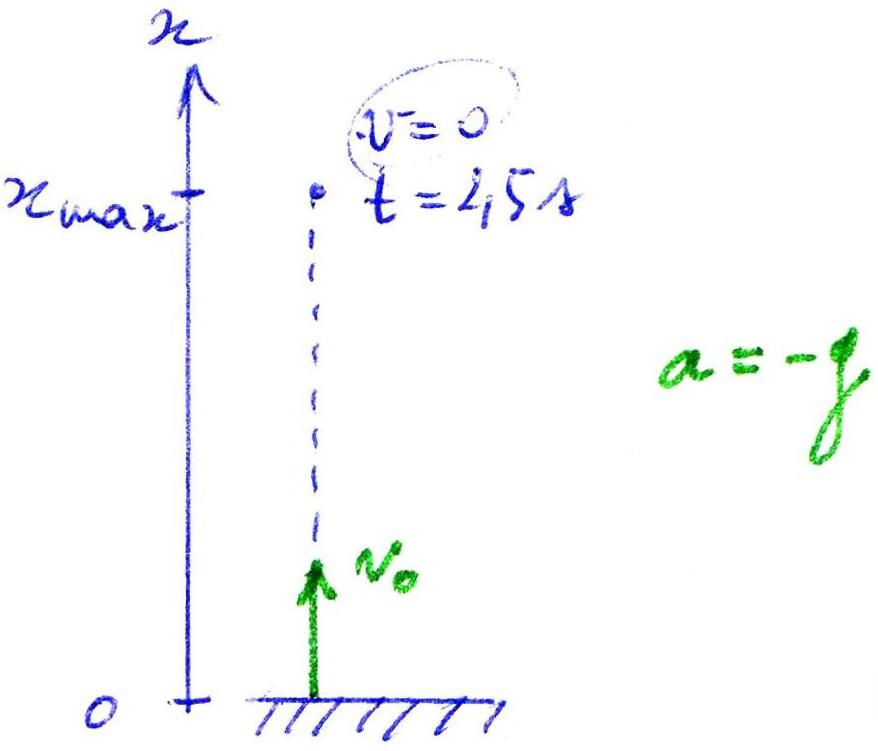
\includegraphics[height=5cm]{55p44}%
	}
\end{minipage}

We krijgen:
\begin{equation*}
v=0\Leftrightarrow v_0-gt=0\Leftrightarrow v_0=gt
\end{equation*}
Dat is in grootte gelijk aan \SI{27}{m/s}.\footnote{Als je voor de valversnelling $g=\SI{10}{m/s^2}$ gebruikt, is de beginsnelheid gelijk aan \SI{28}{m/s}} Nu dat we ook de beginsnelheid kennen, vinden we de afgelegde afstand, wat ook de maximale hoogte is:
\begin{equation*}
x=v_0t-\frac{1}{2}gt^2=(gt)t-\frac{1}{2}gt^2=\frac{1}{2}gt^2
\end{equation*}
Vullen we de getalwaardes in, dan vinden we \SI{38}{m}
\newline
\newline
Merk op dat deze afstand gelijk is aan de afstand die de pijl vanuit rust zou afleggen bij een vrije val die \SI{2,8}{s} duurt. Dat is niet heel verwonderlijk; de vertraging naar boven toe is namelijk gelijk aan de versnelling bij het vallen naar beneden. Wiskundig loopt de symmetrieas van een parabool door de top. 

\end{oplossing} % hoogte
% % !TEX root = ../main.tex



 Aan de rand van een afgrond laat men een steen vallen. Op hetzelfde ogenblik werpt men een steen op. Zou het kunnen dat, als de afgrond diep genoeg is, beide stenen elkaar nog ontmoeten?
\begin{oplossing}
\newline
\newline
Aangezien de opgeworpen steen later (en zelfs hoger) begint met vallen en beide stenen eenzelfde versnelling hebben, kan op geen enkel moment de opgeworpen steen een grotere snelheid hebben dan de steen die wordt losgelaten. Dat laatste zou op het moment van inhalen nochtans op zijn minst het geval moeten zijn.
\newline
\newline
In formules moet gelden, met $v_0$ een negatieve beginsnelheid:
\begin{eqnarray*}
\frac{1}{2}gt^2&=&v_0t+\frac{1}{2}gt^2.
\end{eqnarray*}
Dat is enkel het geval wanneer $t=0$.
\end{oplossing} % Misconceptie ...
% 
\begin{exercise}
% !TEX root = ../main.tex



\pt{10}Een parachutist in vrije val bereikt een uiteindelijke valsnelheid van \SI{50}{m/s}. Neem aan
dat een geopende parachute voor een constante vertraging van \SI{30}{m/s^2} zorgt.\footnote{Dit is een heel ruwe benadering. In feite hangt de vertraging door de parachute namelijk af van de snelheid en is die afhankelijkheid bovendien voor grote snelheden sterker dan voor kleine.} Wil er bij het neerkomen geen kans op letsel bestaan, dan mag de landingssnelheid niet groter dan \SI{5,0}{m/s} zijn. 

Wat is de minimumhoogte voor het openen van de parachute?

\begin{oplossing}
\item[Gegeven]$v_0=\SI{50}{m/s}$\newline$a=\SI{-30}{m/s^2}$\newline$v=\SI{5,0}{m/s}$
\item[Gevraagd]$x$
\item[Oplossing]Aangezien we de versnelling en begin- en eindsnelheid kennen, kunnen we de tijd die nodig is om de eindsnelheid te bereiken, berekenen:
\begin{eqnarray*}
v=v_0+at&\Leftrightarrow&t=\frac{v-v_0}{a}
\end{eqnarray*}
De afgelegde afstand is dan met de gemiddelde snelheid te berekenen:
\begin{eqnarray*}
x&=&\overline{v}t\\
&=&\frac{v_0+v}{2}\cdot\frac{v-v_0}{a}\\
&=&\frac{v^2-v_0^2}{2a}\\
&=&\SI{41,25}{m}
\end{eqnarray*}
\end{oplossing}

\end{exercise}
 % Parachutist
%  Iemand laat een meloen vallen vanop een hoogte van \SI{20}{m}. Op hetzelfde moment schiet je een pijl verticaal omhoog vanop de grond. De pijl treft de meloen na \SI{1,0}{s}. 
\begin{enumerate}
\item Geef in \'e\'en assenstelsel een verzorgde schets van de grafiek van de plaats in functie van de tijd voor beide objecten.
\item Met welke snelheid heb je de pijl afgeschoten? 
\end{enumerate}
\begin{oplossing}
De plaatsfunctie van de meloen gelijkstellen aan die van de afgeschoten pijl, geeft (we kiezen de $y$-as omhoog waardoor de versnelling de negatieve valversnelling is):
\begin{eqnarray*}
y_0-\frac{1}{2}gt^2&=&v_0t-\frac{1}{2}gt^2
\end{eqnarray*}
Oplossen naar $v_0$ geeft: $v_0=\frac{y_0}{t}=\SI{20}{m/s}$.
\end{oplossing} % FV 8 p. 86
% 
\begin{exercise}
% !TEX root = ../main.tex


%[3 p. 90]  
\item\pt{4}\begin{minipage}[t]{.45\linewidth}
Je gooit een bal verticaal omhoog tegen het plafond. De referentie-as staat verticaal omhoog en de grond is de oorsprong. %Hou geen rekening met de versnelling ten gevolge van de botsingen. 
Welk $v(t)$-diagram geeft het best de snelheid van de bal weer? 

\vspace{\baselineskip}
Licht kort toe.
\end{minipage}
\hfill
\begin{minipage}[t]{.5\linewidth}
	\raisebox{1ex-\height}{%
		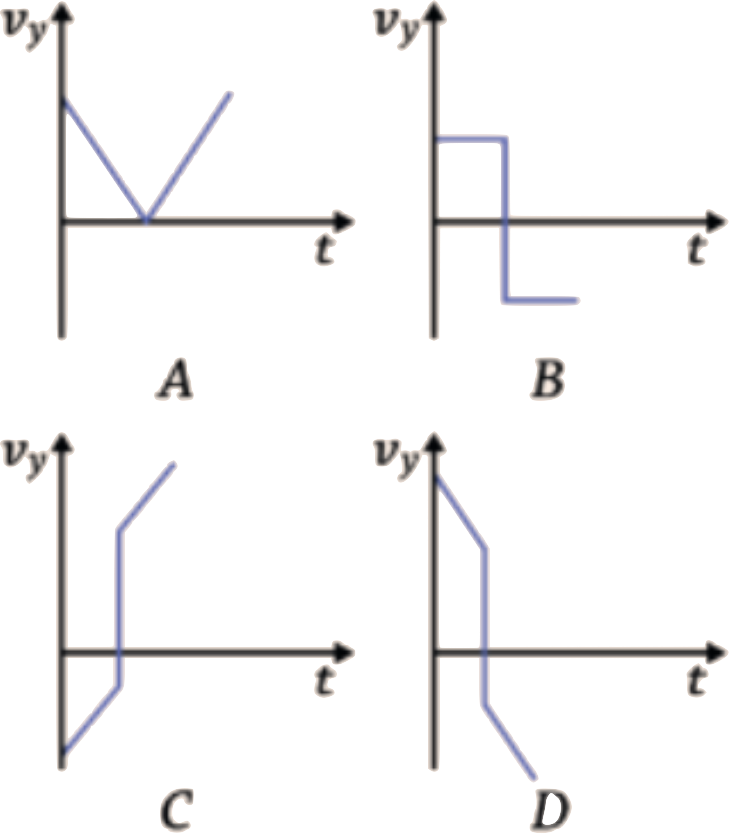
\includegraphics[width=\textwidth]{3p90}} 
\end{minipage}

\begin{oplossing}
D geeft het juiste verloop weer.

Omdat de $y$-as, de as waarmee de beweging beschreven wordt, verticaal omhoog gekozen is, moet de versnellingscomponent negatief zijn. De versnellingsvector is immers naar beneden gericht. De beginsnelheid is met de as mee en dus positief. Omdat de versnelling constant is, moet de snelheid lineair afnemen. Aan deze inzichten voldoen enkel A en D.

Bij de botsing tegen het plafond moet de bal op een hele korte tijd tot stilstand komen om vervolgens op een hele korte tijd weer een even grote snelheid te krijgen, maar nu naar benden. Bij het terug naar beneden komen is de snelheid(svector) tegengesteld gericht aan de as, zodat de component ervan negatief moet zijn. Aan deze beschrijving voldoet enkel D.

\end{oplossing}

\end{exercise}
 %FV 3 p. 90
% 
\begin{exercise}
% !TEX root = ../main.tex



 Wanneer de pelikaan naar vis duikt, trekt hij zijn vleugels in om als een steen loodrecht naar beneden te vallen. 

Stel een pelikaan duikt vanaf \SI{25}{m} hoogte en verandert onderweg dus niet meer van koers. Als het een vis \SI{0,15}{s} kost om te vluchten, wat is dan de hoogte waarop de vis de pelikaan minstens moet opmerken, wil de vis nog kans maken te ontsnappen? 

Neem aan dat de vis zich aan het wateroppervlak bevindt.

\begin{oplossing}
\item[Gegeven]$x_2=\SI{25}{m}$\newline$\Delta t=\SI{0,15}{s}$
\item[Gevraagd]$x_2-x_1$
\item[Oplossing]We kiezen de referentie-as naar beneden, met de oorsprong op de positie waar de pelikaan begint aan zijn duik. De versnelling is dan gelijk aan de valversnelling. 

We kennen de afstand waarover de pelikaan valt zodat we de tijd die de pelikaan nodig heeft om het wateroppervlak te bereiken, de valtijd, kunnen berekenen uit $x_2=\frac{1}{2}gt_2^2 $:
\begin{eqnarray*}
t_2=\sqrt{\frac{2x_2}{g}}
\end{eqnarray*}
De pelikaan heeft namelijk geen beginsnelheid.%De referentie-as is hierbij naar beneden gekozen, met de oorsprong daar waar de pelikaan begint te vallen.

Gedurende een tijd $t_1=t_2-\Delta t$ (15 honderdste van een seconde minder) mag de pelikaan vallen zonder door de vis te worden opgemerkt. De afstand boven het wateroppervlak is dan:
\begin{eqnarray*}
x_2-x_1&=&x_2-\frac{1}{2}gt_1^2\\
&=&x_2-\frac{1}{2}g\left(t_2-\Delta t\right)^2\\
%&=&x_2-\frac{1}{2}g\left(\sqrt{\frac{2x_2}{g}}-\Delta t\right)^2\\
%&=&\Delta t\sqrt{2gx_2}-\frac{1}{2}g\Delta t^2\\
&=&\SI{3,2}{m}
\end{eqnarray*}
\end{oplossing} 

\end{exercise}
 % Pelikaan die naar vis duikt
% % !TEX root = ../main.tex



\item Op de maan is de versnelling van de zwaartekracht slechts een zesde van die op de aarde. Als een voorwerp op de maan verticaal omhoog wordt gegooid, hoeveel maal hoger komt het dan dan een voorwerp dat met dezelfde beginsnelheid vanaf de aarde wordt opgeworpen?

\begin{oplossing}
De tijd die het voorwerp nodig heeft om tot zijn hoogste punt ($v=0$) te geraken, is $t=-\frac{v_0}{a}$ waarbij $a$ de negatieve versnelling op aarde of op de maan is. Met deze tijd en de gemiddelde snelheid gedurende de opwaartse beweging, kunnen we de bereikte hoogte uitdrukken in functie van de beginsnelheid $v_0$:
\begin{eqnarray*}
x=\bar{v}t=\frac{v_0+v}{2}\cdot\left(-\frac{v_0}{a}\right)=-\frac{v_0^2}{2a}
\end{eqnarray*}
Uit deze uitdrukking volgt dat de bereikte hoogte omgekeerd evenredig is met de versnelling. Op de maan zal het voorwerp dan ook zes keer zo hoog geraken.
\end{oplossing} % Maximale hoogte op de maan
% 
\begin{exercise}
% !TEX root = ../main.tex


\pt{10}Een verticaal vallende steen legt in de laatste seconde, voor hij de grond bereikt, \SI{100}{m} af. Men veronderstelt dat hij vanuit rust vertrok.
\begin{enumerate}
\item Bepaal de snelheid op het ogenblik dat hij de grond bereikt.
\item Bepaal de hoogte vanwaar de steen viel en de tijd die hij daarvoor nodig had.
\end{enumerate}

\begin{oplossing}
%\footnote{$v=\frac{x_2-x_1}{t_2-t_1}+\frac{1}{2}g(t_2-t_1)=\frac{\Delta x}{\Delta t}+\frac{1}{2}g\Delta t$
%\newline
%$t_2=\frac{v_2}{g}=\frac{\Delta t}{2}+\frac{\Delta x}{g\Delta t}$, $x=\frac{1}{2}gt^2=\frac{1}{2g}\left(\frac{\Delta x}{\Delta t}\right)^2+\frac{\Delta x}{2}+\frac{g(\Delta t)^2}{8}$}
\item[\textit{gegeven}]$\Delta t=1,0\rm\,s$; $\Delta x=100\rm\,m$; $v_0=0$
\item[\textit{gevraagd}]$v_2$, $x_2$, $t_2$
\item[\textit{oplossing}]
\begin{enumerate}
\item 
\begin{minipage}[t]{.7\textwidth}
We kiezen de $x$-as naar beneden zodat de versnelling de valversnelling is, $a=g$. Als we $x_1$ beschouwen als de beginpositie van de beweging die de steen uitvoert in de laatste honderd meter, kunnen we de snelheid vinden waarmee de steen hieraan `begint'.
\begin{eqnarray*}
&&\Delta x=v_1\Delta t+\frac{1}{2}g\Delta t^2\\
&\Leftrightarrow&v_1=\frac{\Delta x-\frac{1}{2}g\Delta t^2}{\Delta t}
\end{eqnarray*}
\end{minipage}
\begin{minipage}[t][4.5cm][b]{.3\textwidth}
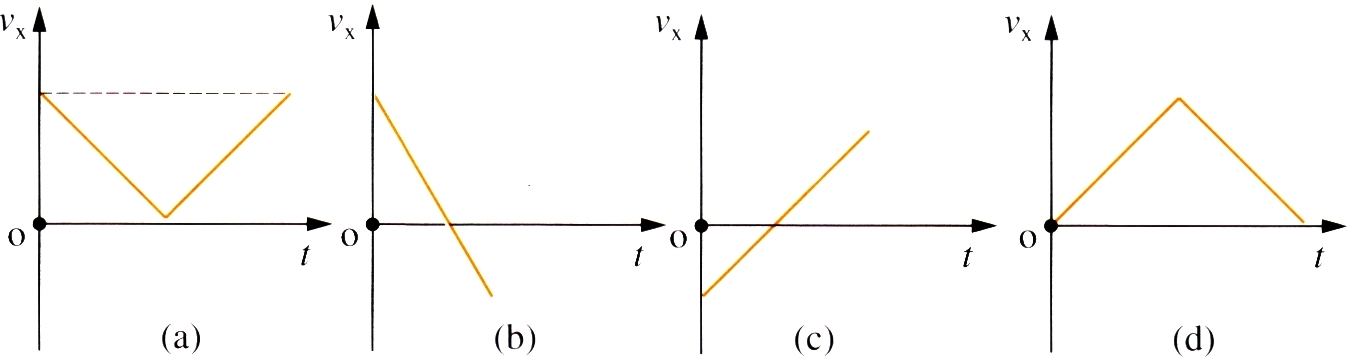
\includegraphics[height=6cm]{valbeweging}
\end{minipage}
\newline
\newline
\newline
Met de formule voor de snelheid van een EVRB, vinden we de snelheid op het einde van het interval.
\begin{eqnarray*}
v_2&=&v_1+g\Delta t\\
&=&\frac{\Delta x-\frac{1}{2}g\Delta t^2}{\Delta t}+g\Delta t\\
&=&\cdots\\
&=&\overline{v}+g\frac{\Delta t}{2}\\
&=&\SI{105}{m/s}
\end{eqnarray*}
Je kan dit ook afleiden door gebruik te maken van de formule voor gemiddelde snelheid, $\overline{v}=\frac{v_1+v_2}{2}$.
\item Omdat we de snelheid kennen, kunnen we de tijd vinden die de steen nodig heeft gehad om aan deze snelheid te komen. Vervolgens vinden we dan ook de afstand.
\begin{eqnarray*}
t_2=\frac{v_2}{g}=\frac{\overline{v}}{g}+\frac{\Delta t}{2}=\SI{10,7}{s}\\
x_2=\frac{1}{2}gt_2^2=\SI{561}{m}
\end{eqnarray*}
\end{enumerate}
\end{oplossing}

\end{exercise}
 % Laatste 100 m
% % !TEX root = ../main.tex



% FV 2 p.  92
%[2 p. 92] 
\item Van de Empire Stage Building in New York komt op \SI{250}{m} een ijskegel los en valt naar beneden.
\begin{enumerate}
\item Na hoeveel tijd en met welke snelheid bereikt het ijskegeltje uiteindelijk de grond?
\item Hoelang en over welke afstand moet de ijskegel al gevallen zijn om in de daaropvolgende \SI{2}{s} een afstand te kunnen afleggen van \SI{100}{m}?
\end{enumerate}
\begin{oplossing}
\item[Gegeven]$x_3=\SI{250}{m}$\newline$\Delta t=t_2-t_1=\SI{2,0}{s}$\newline$\Delta x=x_2-x_1=\SI{100}{m}$
\item[Gevraagd]$t_3,v_3,t_1$ en $x_1$
\item[Oplossing]
\begin{enumerate}

\item\begin{minipage}[t]{0.63\linewidth}
	Omdat de beweging enkel naar beneden is, is de beschrijving gemakkelijk met een $x$-as naar beneden gericht. De versnellingscomponent $a$ is dan gelijk aan de valversnelling $g$. Omdat de kegel vanuit rust vertrekt, vinden we de valtijd uit $x=\frac{1}{2}gt^2$:
\begin{equation*}
t=\sqrt{\frac{2x}{g}}
\end{equation*}
De valtijd bepaalt de eindsnelheid:
\begin{equation*}
v=gt=g\sqrt{\frac{2x}{g}}=\sqrt{2gx}
\end{equation*}
\end{minipage}%
\begin{minipage}[t]{0.37\linewidth}
	\raisebox{1ex-\height}{%
	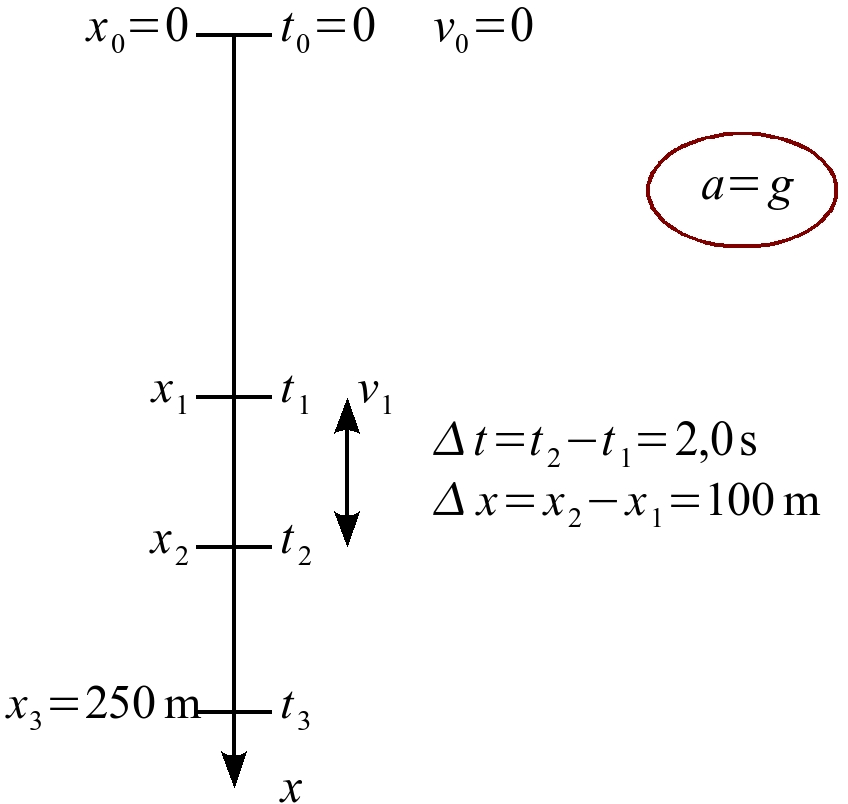
\includegraphics[height=5cm]{opdr16p28}%
	}
\end{minipage}

Invullen van de gegevens geeft $t_3=\SI{7,1}{s}$ en $v_3=\SI{70}{m/s}=\SI{252}{km/h}$.

\item Uit de plaatsfunctie kunnen we de beginsnelheid\footnote{Voor de honderd meter is de beginsnelheid $v_1$.} halen. De beginsnelheid $v_1$ is immers de enige onbekende in de vergelijking:\footnote{Hoe komen we aan deze uitdrukking? De plaatsfunctie toegepast op de honderd meter geeft: $x_2=x_1+v_1t+\frac{1}{2}gt^2$ waarin de variabele $t$ de verstreken tijd tussen tussen de posities $x_1$ en $x_2$ weergeeft. In dit geval stellen we die echter voor door $\Delta t$. Ook is $\Delta x=x_2-x_1$.}
\begin{equation*}
\Delta x=v_1\Delta t+\frac{1}{2}g\Delta t^2\\
\end{equation*}
Dus: $v_1=\frac{2\Delta x-g\Delta t^2}{2\Delta t}$.\footnote{Als we de uitdrukking uitwerken: $v_1=\frac{2\Delta x-g\Delta t^2}{2\Delta t}=\frac{\Delta x}{\Delta t}-g\frac{\Delta t}{2}=\bar{v}-g\frac{\Delta t}{2}$, is te zien dat $v_1$ \'e\'en seconde eerder dan de gemiddelde snelheid bereikt wordt. De gemiddelde snelheid is immers $\bar{v}=\frac{v_1+v_2}{2}$ en wordt dus halverwege de valtijd van de honderd meter bereikt. Bovendien toont deze uitwerking dat we het vraagstuk ook anders hadden kunnen oplossen. Uit $\frac{\Delta x}{\Delta t}=\frac{v_1+v_2}{2}=\frac{v_1+(v_1+g\Delta t)}{2}$ is immers $v_1$ te bepalen.}
%\begin{equation*}
%v_1=\frac{2\Delta x-g\Delta t^2}{2\Delta t}%\\
%%&=&\frac{\Delta x}{\Delta t}-g\frac{\Delta t}{2}\\
%%&=&\bar{v}-g\frac{\Delta t}{2}
%\end{equation*}
%\end{minipage}%
%\begin{figure}[h]
%\centering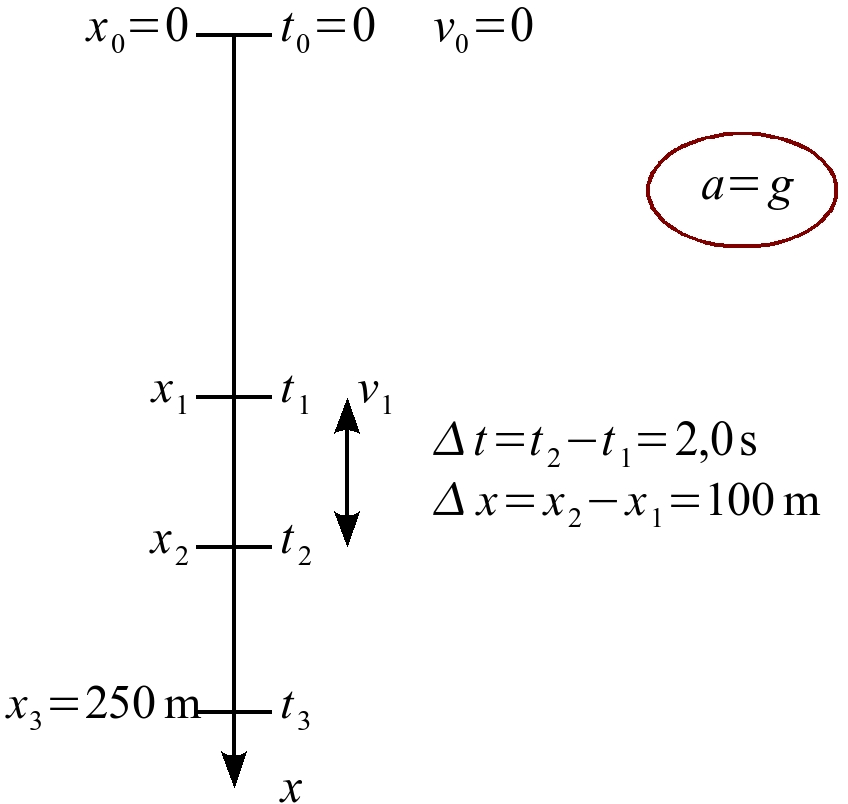
\includegraphics[width=0.4\textwidth]{opdr16p28}
%\end{figure}
Omdat de kegel vanuit rust begint te vallen en per seconde \SI{9,81}{m/s} sneller valt, vinden we de valtijd als $t_1=\frac{v_1}{g}$:
\begin{eqnarray*}
%\Delta x&=&v_1\Delta t+\frac{1}{2}g\Delta t^2\\
%&\Downarrow&(v_1=gt_1)\\
%&=&gt_1\Delta t+\frac{1}{2}g\Delta t^2\\
%&\Updownarrow&\\
t_1=\frac{2\Delta x-g\Delta t^2}{2g\Delta t}&=&\frac{2\cdot100\rm\,m-9,81\rm\,m/s^2\cdot(2,0\rm\,s)^2}{2\cdot9,81\rm\,m/s^2\cdot2,0\rm\,s}=4,1\,s
\end{eqnarray*}
De bijbehorende afgelegde weg is dan $x_1=\frac{1}{2}gt_1^2=82\rm\,m$.
\end{enumerate}
\end{oplossing} % FV 2 p. 92 Empire State Building
% % !TEX root = ../main.tex


\item\pt{10}Een ziek man zit voor een raam dat \SI{1,20}{m} hoog is. Een steen wordt vanop de grond opgeworpen en passeert het raam een keer opwaarts en een keer neerwaarts. De man ziet de steen in totaal voor \'e\'en seconde.% (Een halve bij het opgaan en een halve bij het terug naar beneden gaan.)
\begin{enumerate}
\item Bepaal de snelheid waarmee de steen de onderkant van het raam bereikt.% (die is op het teken na hetzelfde in zowel de opwaartse als de neerwaartse beweging).
\item Toon aan dat het met deze gegevens niet mogelijk is te berekenen hoe hoog het raam boven de grond is gelegen.
\end{enumerate}

\begin{oplossing}
	(a) $\Delta x= v_1\Delta t-\frac{1}{2}g\Delta t^2$ zodat $v_1=\bar{v}+g\frac{\Delta t}{2}=\SI{4,85}{m/s}$ ($\Delta t = \SI{0,5}{s}$)
	
	(b) Naast de hoogte van het raam boven de grond, zijn ook de benodigde tijd en de beginsnelheid onbekende grootheden. Met maar twee vergelijkingen die een EVRB beschrijven ($x=x_0+v_0t+\frac{1}{2}at^2$ en $v=v_0+at$), zijn deze onbekenden niet vast te leggen. 
	
	In een meer fysische uitleg kan je je realiseren dat eenzelfde snelheid aan de onderkant van het raam voor een grotere hoogte boven de grond te realiseren is met een grotere snelheid waarmee de steen opgeworpen wordt.
\end{oplossing}



 % Ziek man voor een raam
% % !TEX root = ../main.tex


\pt{10}Een student gooit een sleutelbos verticaal omhoog naar een medebewoonster in een raam \SI{4,00}{m} hoger. De sleutels worden \SI{1,50}{s} later opgevangen.
\begin{enumerate}
\item Wat was de snelheid waarmee de sleutels omhoog werden gegooid?
\item Welke snelheid had de sleutelbos vlak voordat hij werd opgevangen?
\end{enumerate}

\begin{oplossing}
$v_0=\frac{x+\frac{1}{2}gt^2}{t}=10,02\rm\,m/s$ 

$v=v_0-gt=\frac{x}{t}-\frac{1}{2}gt=\SI{-4,69}{m/s}$
\end{oplossing} % Student gooit een sleutelbos
% 
\begin{exercise}
% !TEX root = ../main.tex



 Een voorwerp wordt verticaal omhoog geworpen en bereikt na een tijd $t$ een hoogte $h$. Toon aan dat de maximale hoogte $h_{\text{max}}$ die het voorwerp bereikt, wordt gegeven door:
\begin{eqnarray*}
h_{\text{max}}&=&\frac{(gt^2+2h)^2}{8gt^2}.
\end{eqnarray*}
\begin{oplossing}
\item[oplossing]We zoeken eerst een uitdrukking voor de maximale hoogte. Op het hoogste punt is de snelheid nul zodat:
\begin{eqnarray*}
v&=&0\\
&\Updownarrow&\\
v_0-gt&=&0\\
&\Updownarrow&\\
t&=&\frac{v_0}{g}
\end{eqnarray*}
Deze tijd is dus de tijd die het voorwerp nodig heeft om het hoogste punt te bereiken. Als we de oorsprong van de $y$-as op de grond kiezen en naar boven gericht, dan vinden we de maximale hoogte door dit tijdstip in de plaatsfunctie in te vullen:
\begin{eqnarray*}
y_{max}&=&y(t_{max})\\
&=&v_0\cdot\left(\frac{v_0}{g}\right)-\frac{1}{2}g\left(\frac{v_0}{g}\right)^2\\
&=&\frac{v_0^2}{2g}
\end{eqnarray*}
Doordat we weten hoe hoog het voorwerp zich bevindt na een tijd $t_1$, kunnen we de beginsnelheid $v_0$ bepalen:
\begin{eqnarray*}
y_1&=&v_0t_1-\frac{1}{2}gt_1^2\\
&\Updownarrow&\\
v_0&=&\frac{2y_1+gt_1^2}{2t_1}
\end{eqnarray*}
Substitutie hiervan in de uitdrukking voor de maximale hoogte geeft de te bewijzen uitdrukking.
\end{oplossing}

\end{exercise}
 % formule voor maximale hoogte





\end{document}

